Así como el propósito de un libro es ser leído y su éxito se mide en la cantidad de personas que lo lean, el éxito de un sitio web informativo se mide en su crecimiento; vive para tener una relación simbiótica con sus usuarios, donde ellos proveen el contenido y con él atraen lectores que se convierten en editores y en nuevos creadores. El sitio web por su parte, aporta todas las herramientas necesarias para que todos puedan participar.

Con el tiempo, y si los usuarios tienen una experiencia positiva este "libro" web, se puede esperar que esté convertido en ecosistema de datos. Para garantizar una buena experiencia de usuario Petter Morville \cite{UXFactors} propone tener en cuenta siguientes factores:

\begin{itemize}
  \item Utilidad: el producto realizado debe ser de utilidad para el público objetivo.
  \item Usabilidad: debe ser un sistema que sea simple y fácil de usar para el usuario.
  \item Deseabilidad: cuando un producto es deseable, los usuarios se sienten atraídos a él.
  \item Encontrable: se debe construir un sistema que sea navegable e instintivo al recorrer, de tal forma que los usuarios puedan encontrar lo que necesiten fácilmente.
  \item Accesibilidad: el sistema debe poder ser usado por la mayor cantidad de personas posibles.
  \item Credibilidad: el sistema debe proporcionar seguridad al usuario acerca de la credibilidad de su contenido
  \item Valor: una experiencia de usuario valiosa implica un buen uso de los demás factores.
\end{itemize}

En este capítulo presentaremos todas las herramientas que nos facilitarán lograr la mejor experiencia de usuario.

\section{Arquitectura}

Para que una aplicación sea encontrable — y así usada — por internautas es fundamental que tenga una buena relación con los motores de búsqueda.

Sin embargo también para asegurar la larga vida y mantenibilidad de la aplicación y la facilidad de desarrollo se debe tomar en cuenta herramientas extensamente empleadas contemporáneamente como Angular, React y Vue.

El problema entonces recae en que estas tecnologías por si solas son meramente para aplicaciones de una sola página. Los motores de búsqueda hacen lo que pueden pero el HTML estático manejado por las SPA es mínimo, resultando en que los motores de búsqueda no puedan inferir de qué trata la página, afectando su habilidad de ser encontrada e indexada.

Como remedio surge un nuevo paradigma con el nombre de Server Side Rendering o simplemente SSR \cite{ServerSideRendering}; donde se utilizan  tecnologías SPA como motor de plantillas, para así generar HTML digerible por los motores de búsqueda. Una vez el HTML estático llega al cliente, este atraviesa un proceso conocido como \textit{hydration}, donde retoma sus funcionalidades dinámicas características de SPA.

Así se logra el perfecto balance de herramientas actuales y fáciles de usar, que también cumplen con los requerimientos de los motores de búsqueda para indexar páginas web.

\section{Tecnologías para el desarrollo}

Actualmente existe un catálogo muy amplio de tecnologías de desarrollo web, por lo que escoger las debidas herramientas y analizar sus compatibilidades es clave para obtener el mejor conjunto de herramientas.

El este capítulo hablaremos de las herramientas de desarrollo web usadas para llevar a cabo el proyecto, y las descompondremos en 2 categorías: Servidor y Cliente.

\section{Servidor}

\subsection{Fastify}

Fastify es un framework web para NodeJS de código abierto concentrado en proporcionar el mejor rendimiento, y una arquitectura flexible. 

Las principales características de Fastify son \cite{FastifyCoreFeatures}:

\begin{itemize}
    \item Alto rendimiento: si se compara la velocidad de Fastify con otros frameworks web como Express, tal como se aprecia en la figura \ref{fig:fastify_vs_express}, notamos que Fastify es aproximadamente un 20\% más rápido que Express.
    \item Extensible: Fastify es completamente extensible mediante el uso de \textit{hooks}, plugins o decoradores.
    \item Basado en esquemas: a pesar de no ser obligatorio, es recomendado usar el esquema JSON para validar las rutas y serializar las salidas, internamente Fastify compila el esquema en una función de alto rendimiento.
    \item Registro: Usualmente el guardar un registro puede ser costoso, por esa razón Fastify hace uso de un logger eficiente que casi remueve ese costo.
    \item Amigable para los desarrolladores: este framework está desarrollado para ser bastante expresivo y ayudar a los desarrolladores en su uso, sin sacrificar rendimiento o seguridad.
    \item Listo para usar con Typescript: la instalación inicial del framework provee compatibilidad predeterminada con Typescript
\end{itemize}


\begin{figure}[H]
    \centering
    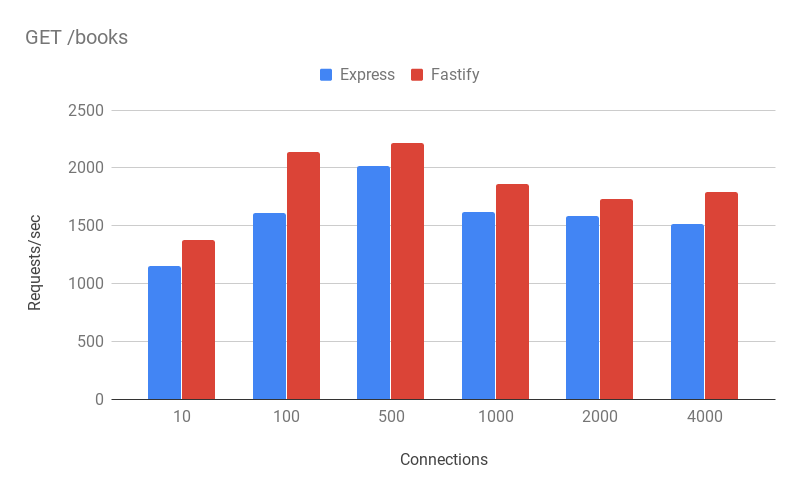
\includegraphics[width=\textwidth]{fastify_vs_express.png}
    \caption{ Número de peticiones por segundo para distinta cantidad de conexiones}
    \label{fig:fastify_vs_express}
\end{figure}

\subsection{MongoDB}

MongoDB es un sistema manejador de base de datos de documentos NoSQL escalable y flexible diseñado para lidiar con los conflictos que poseen las bases de datos relacionales y las limitaciones de otras soluciones NoSQL. En lugar de guardar los datos en tablas, tal y como se hace en las bases de datos relacionales, MongoDB guarda estructuras de datos BSON (una especificación similar a JSON) con un esquema dinámico, lo que facilita la integración de los datos.

No tener restricciones al estructurar los datos facilita el desarrollo, siempre y cuando el desarrollador sea consciente de la redundancia que puede causar en la base de datos. Los documentos BSON almacenados en colecciones dentro de MongoDB, estos son similares al conocidísimo estándar JSON. Las consultas y mutaciones en MongoDB no son hechas en un lenguaje de consulta como SQL sino serializadas en JSON.

Como se puede observar en la imagen \ref{fig:ranking-db}, mongoDB es actualmente la opción más usada entre las bases de datos NoSQL, ocupando el puesto número 5 en el ranking de bases de datos propuesto por Stack Overflow \cite{StackOverflowSurvey}. Esto proporciona suficiente certeza de que MongoDB será mantenido por años en el futuro.

\begin{figure}[H]
    \centering
    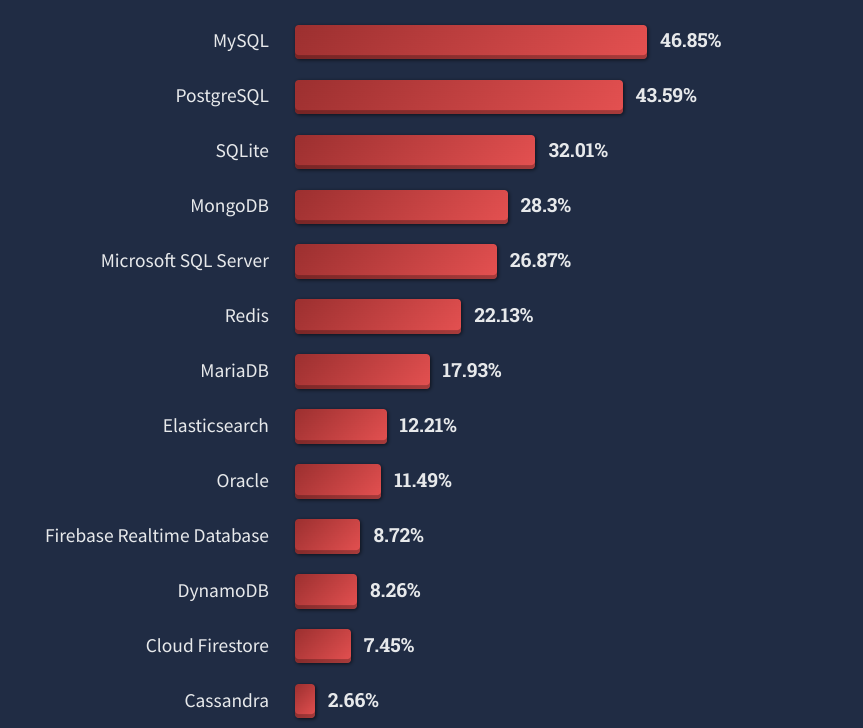
\includegraphics[width=\textwidth]{ranking-db.png}
    \caption{Ranking de bases de datos más populares de 2022}
    \label{fig:ranking-db}
\end{figure}

Algunas de las características más importantes de MongoDB son:

\begin{itemize}
  \item Consultas ad-hoc optimizadas para análisis en tiempo real
  \item Indexación adecuada para mejores tiempos de ejecución de consultas
  \item Replicación para una mejor disponibilidad y estabilidad de los datos
  \item \textit{Sharding}\footnote{\textit{Sharding}: proceso de distribuir un conjunto de datos en múltiples bases de datos, que después pueden ser almacenados en múltiples ordenadores.}
  \item Balanceo de carga
\end{itemize}

Para realizar operaciones sobre la base de datos MongoDB usando un servidor NodeJS es necesario usar un MongoDB Driver compatible con NodeJS, el cual permite establecer una conexión con la base de datos, y que provee una API que facilita la interacción con la misma. A continuación se mostrará un código básico de conexión y consulta de datos usando el NodeJS MongoDB Driver.

\begin{lstlisting}
    import { MongoClient } from "mongodb";

    const uri = "<connection string uri>";

    const client = new MongoClient(uri);

    async function run() {

        await client.connect();

        const database = client.db("sample_mflix");

        const movies = database.collection("movies");

        const query = { title: "The Room" };

        const options = {};

        const movie = await movies.findOne(query, options);

    }
\end{lstlisting}

En el código se puede observar como se utiliza el cliente de MongoDB para conectarse a la base de datos \textquote{sample\_mflix} y después consultar todas las películas cuyo título sea igual a \textquote{The Room}.

\section{Cliente}

Para este proyecto se usarán las siguientes tecnologías:

\subsection{ReactJS}

ReactJS es una librería de JavaScript de código abierto desarrollada por Facebook para facilitar la creación de componentes interactivos y reutilizables, para desarrollo de interfaces de usuario, especialmente aplicaciones de una sola página.

React maneja el concepto de \say{programación reactiva} \cite{ReactiveProgramming} haciendo uso de un DOM Virtual, lo que le permite determinar qué partes del DOM han cambiado comparando contenidos entre la versión nueva y la almacenada en el DOM virtual, para así propagar los datos generando cambios en la aplicación, es decir, la aplicación \say {reacciona} a cambios en los datos ejecutando una serie de eventos y re-renderizando solo aquellos componentes que lo ameriten. Esto es el secreto de porqué React es altamente eficiente.

Otras características que destacan en React son:

\begin{itemize}
  \item \textbf{Componentes} \hfill

        El código de React es hecho con entidades llamadas componentes. Los componentes pueden ser renderizados en elementos particulares del DOM usando la librería de React DOM. Estos componentes son capaces de recibir parámetros conocidos como "propiedades del componente" de la siguiente forma: \hfill 

        \begin{lstlisting}
            ReactDOM.render(<Greeter greeting="Hello World!" />, document.getElementById('myReactApp'));
        \end{lstlisting}

        Las 2 formas de declarar componentes en React es mediante el uso de funciones o clases, y generalmente se usa una de las dos opciones de forma situacional.

  \item \textbf{JSX} \hfill

        JSX, también llamado Javascript XML, es una extension a la sintaxis del lenguaje javascript. Este provee una forma de estructurar componentes usando una sintaxis familiar para muchos desarrolladores. Los componentes de React son usualmente escritos en JSX, aunque también pueden ser escritos usando Javascript puro.

        Un ejemplo de código JSX:

        \begin{lstlisting}
            class App extends React.Component {
                render() {
                    return (
                    <div>
                        <p>Header</p>
                        <p>Content</p>
                        <p>Footer</p>
                    </div>
                    );
                }
            }
        \end{lstlisting}

  \item \textbf{Hooks} \hfill 

        Los hooks son funciones que permiten a los desarrolladores \say{engancharse} a los estados de React y a ciertos puntos dentro del ciclo de vida de los componentes.

        React proporciona algunos hooks integrados tales como: useState, useContext, useReducer, useMemo y useEffect son los más usados y permiten controlar los estados y manejar eventos.
\end{itemize}

\subsection{Next.js}

Next.js es un framework desarrollado sobre NodeJS que permite a las aplicaciones de React usar funcionalidades como el renderizado del lado servidor y la generación de páginas web estáticas.

Por defecto, Next.js pre-renderiza cada página. Esto significa que Next.js genera HTML para cada página en adelanto, en vez de hacerse con Javascript del lado del cliente. Pre-renderizado puede resultar en mejor rendimiento y SEO.

Cada HTML generado es asociado con el mínimo código Javascript necesario para que funcione la página. Cuando una página es cargada en el explorador, su código javascript se ejecuta y hace la página totalmente interactiva. A este proceso de le conoce como \say{hydration}

Next.js ofrece 2 formas de pre-renderizado:

\begin{itemize}
  \item Generación estática: El HTML es pre-generado y puede ser servido estáticamente.
  \item Renderizado del lado servidor: El HTML es generado al recibir una petición del cliente, necesita un servidor que procese las peticiones.
\end{itemize}

\subsection{Material UI}

Material UI es un framework de React creado con el objetivo de proporcionar una forma sencilla a los desarrolladores de aplicar los principios de Material Design \cite{MaterialDesignPrinciples} usando componentes de React. Este framework se destaca por la gran variedad de componentes disponibles, que van desde elementos visuales sencillos como botones o selectores, hasta complejos como modales o drawers. Además de su variedad de componentes, Material UI también destaca por su gran cantidad de contribuyentes, lo que asegura la longevidad y mantenibilidad del framework.

Entre las principales características que posee Material UI se encuentran:

\begin{itemize}
  \item Posibilidad de crear temas, lo que permite personalizar los estilos predeterminados de los componentes de la librería de forma global, o acotada.
  \item Construido usando la estrategia Mobile First \cite{MobileFirst}, en la cual se crea el código primero para dispositivos móviles, y después se escalan usando las reglas de CSS pertinentes.
  \item Los componentes de Material UI se consideran autosuficientes, por lo que solo utilizan los estilos CSS necesarios para mostrar el componente en pantalla, es decir, no dependen de hojas de estilos globales como en el caso de normalize.css o bootstrap.
\end{itemize}

A continuación se mostrará el uso de algunos componentes que ofrece la librería:

\begin{itemize}
  \item Botones

        \begin{lstlisting}
                <Button variant="text">Text</Button>
                <Button variant="contained">Contained</Button>
                <Button variant="outlined">Outlined</Button>
                <Button color="secondary">Secondary</Button>
                <Button size="small">Small</Button>
                <IconButton aria-label="delete">
                    <DeleteIcon />
                </IconButton>
            \end{lstlisting}

        Material UI viene incluido con 3 variantes visuales de botones, los cuales son usados dependiendo de la importancia o énfasis que se le quiera dar al botón. Además, también posee variaciones de color y tamaño predeterminados y la posibilidad de usar íconos que funcionan como botones.

  \item Selectores

        \begin{lstlisting}
                <FormControl fullWidth>
                    <InputLabel id="demo-simple-select-label">Age</InputLabel>
                    <Select
                        labelId="demo-simple-select-label"
                        id="demo-simple-select"
                        value={age}
                        label="Age"
                        onChange={handleChange}
                    >
                        <MenuItem value={10}>Ten</MenuItem>
                        <MenuItem value={20}>Twenty</MenuItem>
                        <MenuItem value={30}>Thirty</MenuItem>
                    </Select>
                </FormControl>
            \end{lstlisting}

        El selector comúnmente se encuentra envuelto en un componente de FormControl, el cual provee contexto para hacer uso de campos requeridos, manejo de errores y uso de propiedades como "seleccionado" o "campo lleno".

  \item Sliders

        \begin{lstlisting}
                const marks = [
                    {
                        value: 0,
                        label: "0km"
                    },
                    {
                        value: 20,
                        label: "20km"
                    },
                    {
                        value: 37,
                        label: "37km"
                    },
                    {
                        value: 100,
                        label: "100km"
                    },
                ];
                <Slider aria-label="Volume" value={25} onChange={handleChange} />
                <Slider defaultValue={30} step={10} marks min={10} max={110} disabled />
                <Slider
                    aria-label="Custom marks"
                    defaultValue={20}
                    getAriaValueText={valuetext}
                    step={10}
                    valueLabelDisplay="auto"
                    marks={marks}
                />
            \end{lstlisting}

        Material UI permite personalizar los Sliders de múltiples maneras, tales como usar valores discretos, cambiar el tamaño del Slider, o utilizar íconos personalizados en los extremos o en la perilla de este, lo que contextualiza al usuario sobre lo que representa el valor del Slider.

\end{itemize}

